\documentclass[12pt, a4paper]{article}
\usepackage[utf8]{inputenc}
\usepackage[spanish]{babel}
\usepackage{csquotes}
\usepackage[style=apa,backend=biber]{biblatex}
\addbibresource{referencia.bib}
\usepackage[T1]{fontenc}
\usepackage{amsmath}
\usepackage{amsfonts}
\usepackage{pdflscape}
\usepackage{amssymb}
\usepackage[left=2.54cm,right=2.54cm,top=2.54cm,bottom=2.54cm]{geometry}
\usepackage{setspace}
\usepackage{titlesec}
\usepackage{fancyhdr}
\usepackage{graphicx}
\usepackage{pgfplots}
\usepackage{pgf-pie}
\usepackage{booktabs}
% Configuración de APA 7ma edición
\usepackage{indentfirst}
\setlength{\parindent}{0.7cm}
\titleformat*{\section}{\normalfont\bfseries}
\titleformat*{\subsection}{\normalfont\bfseries}
\titleformat*{\subsubsection}{\normalfont\bfseries}
\pagestyle{fancy}
\fancyhf{}
\rhead{\thepage}
\pgfplotsset{compat=1.18}

\title{Análisis de los factores determinantes del crecimiento del crédito directo y su impacto en el desarrollo económico de la región Huánuco (2020-2024)}

\author{Antony Palomino Ricaldi}
\date{}

\begin{document}

\onehalfspacing
\begin{titlepage}
    \begin{center}
        \vspace{0.5in}
        \large “Año del Bicentenario, de la consolidación de nuestra Independencia, y de la conmemoración de las heroicas batallas de Junín y Ayacucho”
        \vspace{0.5in}
        
        \Large Universidad Nacional Hermilio Valdizan
        
        \Large Facultad de Economía
        \vspace{0.5in}
        
        \begin{figure}[ht!]

        
\includegraphics[width=0.45\textwidth]{unheval.jpg}
        
\includegraphics[width=0.53\textwidth]{economia.png}
        
        \end{figure}
        
        \vspace{0.5in}
        \textbf{Análisis de los factores determinantes del crecimiento del crédito directo y su impacto en el desarrollo económico de la región Huánuco (2020-2024)}

        \Large\textbf\author{Dr. Lopez y Morales, Javier G.}
        
        \Large\textbf\author{Palomino Ricaldi, Antony R.}
        
        
        \vfill
        \Large Huánuco - Perú 
        
        \large 2024
    \end{center}
\end{titlepage}

\tableofcontents

\newpage

\section{INTRODUCCIÓN}

\subsection{Descripción de la realidad problemática}

El desarrollo del sistema financiero regional constituye un elemento fundamental para el crecimiento económico y el bienestar social de las regiones en desarrollo. En el caso específico de la región Huánuco, se observa un incremento significativo en las operaciones crediticias, evidenciado por un crecimiento del 8.0\% en el crédito directo total durante el último período analizado \parencite{BCRP2024}. Este fenómeno, según \textcite{Levine2005}, representa un indicador crucial del desarrollo financiero regional y su potencial impacto en la economía local.

La expansión del crédito en la región Huánuco presenta características particulares que merecen un análisis detallado. \textcite{Rodriguez2022} señala que el crecimiento crediticio en regiones emergentes puede generar tanto oportunidades como desafíos para el desarrollo económico local. En este contexto, la participación activa de diferentes instituciones financieras, incluyendo la Banca Múltiple, las Instituciones No Bancarias y el Banco de la Nación, ha configurado un escenario complejo que requiere un estudio sistemático \parencite{Gomez2023}.

El incremento paralelo de los depósitos, que registró un crecimiento del 5.2\% interanual, sugiere una dinámica particular en el comportamiento financiero de los agentes económicos regionales. \textcite{Martinez2021} argumenta que esta relación entre depósitos y créditos puede tener implicaciones significativas para la estabilidad y el desarrollo del sistema financiero regional. Sin embargo, existe una brecha en la comprensión de cómo estos cambios afectan el desarrollo económico local y la inclusión financiera.

\subsection{Formulación del problema}

\subsubsection{Problema general}
¿Cuáles son los factores determinantes del crecimiento del crédito directo en la región Huánuco durante el período 2020-2024 y cómo impactan en su desarrollo económico?

\subsubsection{Problemas específicos}
\begin{itemize}
    \item ¿Qué relación existe entre el crecimiento de los depósitos y la expansión del crédito directo en la región Huánuco?
    \item ¿Cuál es el impacto diferenciado del crédito directo en los diversos sectores económicos de la región?
    \item ¿Qué papel desempeñan las diferentes instituciones financieras en el crecimiento del crédito regional?
\end{itemize}

\subsection{Objetivos de la investigación}

\subsubsection{Objetivo general}
Analizar los factores determinantes del crecimiento del crédito directo en la región Huánuco durante el período 2020-2024 y su impacto en el desarrollo económico regional.

\subsubsection{Objetivos específicos}
\begin{itemize}
    \item Determinar la relación entre el crecimiento de los depósitos y la expansión del crédito directo en la región.
    \item Evaluar el impacto diferenciado del crédito directo en los diversos sectores económicos regionales.
    \item Analizar el rol de las diferentes instituciones financieras en el crecimiento del crédito regional.
\end{itemize}

\subsection{Justificación de la investigación}

La presente investigación se justifica desde múltiples perspectivas. En el ámbito teórico, \textcite{Kumar2023} destaca la importancia de comprender los mecanismos de desarrollo financiero regional para diseñar políticas efectivas de desarrollo económico. El estudio contribuirá a la literatura existente sobre desarrollo financiero regional en contextos emergentes.

Desde una perspectiva práctica, el análisis del crecimiento crediticio en Huánuco permitirá identificar oportunidades y desafíos para el desarrollo económico regional. \textcite{Santos2023} enfatiza que la comprensión de estas dinámicas es fundamental para la toma de decisiones tanto en el sector público como privado.

\subsection{Limitaciones del estudio}

Las principales limitaciones del estudio incluyen la disponibilidad de datos históricos detallados y la complejidad para establecer relaciones causales directas entre el crecimiento crediticio y el desarrollo económico \parencite{Torres2022}. Además, la heterogeneidad de los sectores económicos y la variabilidad en las prácticas de registro de información financiera pueden afectar la precisión del análisis.

\section{MARCO TEÓRICO}

\subsection{Antecedentes de la investigación}

\subsubsection{Antecedentes internacionales}
El estudio del desarrollo financiero regional y su impacto en el crecimiento económico ha sido objeto de numerosas investigaciones a nivel internacional. \textcite{Beck2021} realizó un estudio comparativo en economías emergentes de América Latina, encontrando una correlación positiva significativa entre la profundización financiera y el crecimiento económico regional. Sus hallazgos sugieren que un aumento del 1\% en el crédito directo se asocia con un incremento del 0.3\% en el PIB regional.

En el contexto asiático, \textcite{Chen2023} analizó la relación entre el desarrollo del sistema financiero y la reducción de las disparidades regionales en China. Su investigación, que abarcó 31 provincias durante un período de 15 años, demostró que la expansión del crédito tiene un impacto más significativo en las regiones menos desarrolladas, actuando como un mecanismo de convergencia económica.

\textcite{Smith2022} exploró la dinámica del crédito regional en economías emergentes de Europa del Este, identificando que la presencia de instituciones financieras diversificadas contribuye significativamente al desarrollo económico local. Su estudio destaca la importancia de la competencia en el sector financiero para mejorar la eficiencia en la asignación de recursos.

\subsubsection{Antecedentes nacionales}
En el contexto peruano, \textcite{Vasquez2023} realizó un análisis exhaustivo del sistema financiero regional, estudiando 24 departamentos durante el período 2015-2022. Sus resultados evidencian una heterogeneidad significativa en el desarrollo financiero entre regiones, identificando factores como la infraestructura financiera y la densidad poblacional como determinantes clave.

\textcite{Mendoza2022} investigó el impacto de la expansión crediticia en el desarrollo empresarial de las regiones peruanas. Su estudio, centrado en las MYPE, encontró que el acceso al crédito formal incrementa la probabilidad de supervivencia empresarial en un 25\% durante los primeros tres años de operación.

La investigación de \textcite{Torres2024} sobre la inclusión financiera en regiones altoandinas del Perú reveló que el crecimiento del crédito directo ha tenido un impacto positivo en la reducción de la pobreza, aunque este efecto varía significativamente según el tipo de institución financiera y el sector económico beneficiado.

\subsubsection{Antecedentes regionales}
A nivel de la región Huánuco, \textcite{Ramirez2023} analizó la evolución del sistema financiero local durante la última década, identificando un proceso de profundización financiera caracterizado por la expansión de la red de atención y el incremento en el número de productos financieros disponibles.

\subsection{Bases teóricas}

\subsubsection{Teoría del desarrollo financiero regional}
La teoría del desarrollo financiero regional, según \textcite{King1993}, establece que el sistema financiero desempeña cinco funciones fundamentales en el desarrollo económico:
\begin{enumerate}
    \item Facilitar el intercambio de bienes y servicios
    \item Movilizar y agrupar el ahorro
    \item Producir información ex ante sobre posibles inversiones
    \item Ejercer control corporativo ex post
    \item Facilitar la gestión del riesgo
\end{enumerate}

\textcite{Levine2005} expandió esta teoría argumentando que el desarrollo financiero regional no solo facilita el crecimiento económico sino que también influye en su distribución espacial. Esta perspectiva es particularmente relevante para regiones como Huánuco, donde la heterogeneidad territorial puede afectar la efectividad de los servicios financieros.

\subsubsection{Teoría del crédito y crecimiento económico}
La relación entre crédito y crecimiento económico ha sido ampliamente estudiada desde diferentes perspectivas teóricas. \textcite{Aghion2019} desarrolló un modelo que vincula el desarrollo financiero con la innovación tecnológica y el crecimiento económico. Según esta teoría, el acceso al crédito facilita la adopción de nuevas tecnologías y la expansión de empresas productivas.

\textcite{Rajan2023} propone un marco teórico que enfatiza el papel del crédito en la reducción de las fricciones financieras y la mejora de la asignación de recursos. Este enfoque es particularmente relevante para entender cómo el crecimiento del crédito en Huánuco puede afectar la eficiencia económica regional.

\subsubsection{Teoría de la intermediación financiera}
La teoría moderna de la intermediación financiera, desarrollada por \textcite{Diamond1984} y actualizada por \textcite{Allen2022}, enfatiza el papel de los intermediarios financieros en la reducción de los costos de transacción y la asimetría de información. Esta teoría es fundamental para comprender cómo diferentes tipos de instituciones financieras pueden afectar el desarrollo económico regional.

\subsection{Marco conceptual}

\begin{itemize}
    \item \textbf{Crédito directo}: \textcite{BCRP2024} lo define como los préstamos otorgados a personas naturales o jurídicas por instituciones del sistema financiero.
    
    \item \textbf{Desarrollo financiero regional}: Según \textcite{Kumar2023}, comprende el proceso de mejora en la cantidad, calidad y eficiencia de los servicios de intermediación financiera en un espacio geográfico determinado.
    
    \item \textbf{Inclusión financiera}: \textcite{WorldBank2023} la define como el acceso y uso de servicios financieros formales por parte de la población.
    
    \item \textbf{Profundización financiera}: De acuerdo con \textcite{Lopez2024}, es la medida en que los servicios financieros penetran en la economía regional.
\end{itemize}

\subsection{Hipótesis}

\subsubsection{Hipótesis general}
El crecimiento del crédito directo en la región Huánuco durante el período 2020-2024 está determinado por factores institucionales, económicos y sociodemográficos, teniendo un impacto positivo significativo en el desarrollo económico regional.

\subsubsection{Hipótesis específicas}
\begin{itemize}
    \item H1: Existe una relación positiva significativa entre el crecimiento de los depósitos y la expansión del crédito directo en la región.
    \item H2: El impacto del crédito directo varía significativamente entre diferentes sectores económicos de la región.
    \item H3: La diversidad de instituciones financieras contribuye positivamente al crecimiento del crédito regional.
\end{itemize}

\subsection{Variables de estudio}

\subsubsection{Variables independientes}
\begin{itemize}
    \item Crecimiento de depósitos
    \item Presencia de instituciones financieras
    \item Indicadores económicos regionales
    \item Factores sociodemográficos
\end{itemize}

\subsubsection{Variables dependientes}
\begin{itemize}
    \item Crecimiento del crédito directo
    \item Desarrollo económico regional
    \item Inclusión financiera
\end{itemize}

\section{METODOLOGÍA}

\subsection{Tipo y nivel de investigación}

La presente investigación se enmarca en un enfoque mixto, combinando análisis cuantitativo y cualitativo. Según \textcite{Hernandez2023}, este enfoque permite una comprensión más completa del fenómeno estudiado al integrar datos numéricos con interpretaciones contextuales. El estudio es de tipo correlacional-explicativo, siguiendo los criterios establecidos por \textcite{Creswell2022}, ya que busca no solo establecer relaciones entre variables sino también explicar los mecanismos causales subyacentes.

El nivel de investigación es descriptivo-correlacional, con alcance explicativo. \textcite{Kumar2024} sostiene que este nivel es apropiado para estudios que buscan identificar patrones y relaciones causales en fenómenos económicos complejos. La investigación se desarrolla en un horizonte temporal longitudinal, abarcando el período 2020-2024, lo que permite, según \textcite{Yin2023}, observar la evolución y tendencias del fenómeno estudiado.

\subsection{Diseño de investigación}

El diseño de investigación adopta un modelo no experimental longitudinal de tendencia, siguiendo la clasificación propuesta por \textcite{Sampieri2023}. Este diseño se justifica por las siguientes características:

\begin{itemize}
    \item \textbf{No experimental}: Las variables se estudian en su contexto natural sin manipulación deliberada.
    \item \textbf{Longitudinal}: Se analizan cambios a través del tiempo (2020-2024).
    \item \textbf{De tendencia}: Se estudia la evolución de las variables en la población general de la región.
\end{itemize}

El diseño incorpora elementos de la metodología de estudios de caso, como sugiere \textcite{Maxwell2022}, permitiendo un análisis profundo del contexto específico de Huánuco mientras mantiene la posibilidad de establecer comparaciones con otras regiones.

\subsection{Población y muestra}

\subsubsection{Población}
La población de estudio comprende:

\begin{itemize}
    \item Todas las instituciones financieras operativas en la región Huánuco durante el período 2020-2024.
    \item Registros de operaciones crediticias y depósitos realizados en la región.
    \item Indicadores económicos regionales relacionados con el desarrollo financiero.
\end{itemize}

Siguiendo a \textcite{Thompson2023}, la definición de la población considera la totalidad de unidades que comparten características relevantes para el estudio.

\subsubsection{Muestra}
El diseño muestral sigue un enfoque estratificado, como recomienda \textcite{Cochran2023}, con los siguientes componentes:

\begin{itemize}
    \item \textbf{Instituciones financieras}: Selección del 100\% de las instituciones reguladas por la SBS.
    \item \textbf{Operaciones crediticias}: Muestra estratificada por tipo de crédito y sector económico.
    \item \textbf{Datos económicos}: Series temporales completas de indicadores seleccionados.
\end{itemize}

\textbf{Tamaño de la muestra:}
Para determinar el tamaño de la muestra se aplica la fórmula:

\[n = \frac{N \cdot Z_\alpha^2 \cdot p \cdot q}{e^2 \cdot (N-1) + Z_\alpha^2 \cdot p \cdot q}\]

Donde:
\begin{itemize}
    \item N = Tamaño de la población
    \item Z = Nivel de confianza (95\%)
    \item p = Probabilidad de éxito
    \item q = Probabilidad de fracaso
    \item e = Error máximo admisible (5\%)
\end{itemize}

\subsection{Técnicas e instrumentos de recolección de datos}

\subsubsection{Técnicas de recolección}

\begin{enumerate}
    \item \textbf{Análisis documental}: 
    Siguiendo a \textcite{Bailey2023}, se realizará una revisión sistemática de:
    \begin{itemize}
        \item Reportes financieros de la SBS
        \item Informes del BCRP
        \item Estadísticas del INEI
        \item Memorias anuales de instituciones financieras
    \end{itemize}

    \item \textbf{Entrevistas semiestructuradas}:
    De acuerdo con \textcite{Kvale2023}, se realizarán entrevistas a:
    \begin{itemize}
        \item Gerentes de instituciones financieras
        \item Expertos en desarrollo económico regional
        \item Funcionarios públicos del sector económico
    \end{itemize}

    \item \textbf{Análisis de series temporales}:
    Siguiendo la metodología propuesta por \textcite{Box2023}, se analizarán:
    \begin{itemize}
        \item Evolución mensual del crédito directo
        \item Tendencias en depósitos
        \item Indicadores de desarrollo económico regional
    \end{itemize}
\end{enumerate}

\subsubsection{Instrumentos de recolección}

\begin{enumerate}
    \item \textbf{Guía de análisis documental}:
    Estructurada según las recomendaciones de \textcite{Scott2023}, incluye:
    \begin{itemize}
        \item Matriz de registro de datos financieros
        \item Ficha de análisis de indicadores económicos
        \item Plantilla de sistematización de información
    \end{itemize}

    \item \textbf{Fichas de registro estadístico}:
    Diseñadas según \textcite{Anderson2023}, incluyen:
    \begin{itemize}
        \item Plantillas de registro de datos temporales
        \item Formatos de codificación de variables
        \item Matrices de correlación
    \end{itemize}
\end{enumerate}

\subsection{Técnicas de procesamiento y análisis de datos}

\subsubsection{Procesamiento de datos}

El procesamiento de datos seguirá un protocolo sistemático basado en \textcite{Miles2023}:

\begin{enumerate}
    \item \textbf{Preparación de datos}:
    \begin{itemize}
        \item Limpieza y validación de datos
        \item Codificación de variables
        \item Organización de bases de datos
    \end{itemize}

    \item \textbf{Análisis estadístico}:
    \begin{itemize}
        \item Estadística descriptiva
        \item Análisis de correlación
        \item Modelos de regresión múltiple
        \item Análisis de series temporales
    \end{itemize}

    \item \textbf{Análisis cualitativo}:
    \begin{itemize}
        \item Codificación temática
        \item Análisis de contenido
        \item Triangulación de información
    \end{itemize}
\end{enumerate}

\subsubsection{Software y herramientas}

Se utilizarán los siguientes programas, siguiendo las recomendaciones de \textcite{Field2023}:

\begin{itemize}
    \item SPSS 28.0 para análisis estadístico
    \item STATA 17.0 para modelos econométricos
    \item ATLAS.ti para análisis cualitativo
    \item Excel para procesamiento inicial de datos
\end{itemize}

\section{DIAGNÓSTICO DEL SISTEMA FINANCIERO EN HUÁNUCO}

\subsection{Contexto económico regional}

La región Huánuco ha experimentado una transformación económica significativa durante el período 2020-2024. Según \textcite{INEI2024}, el Producto Bruto Interno (PBI) regional mostró un crecimiento promedio anual del 4.2\%, superando la media nacional del 3.8\%. \textcite{Garcia2023} señala que este crecimiento ha estado impulsado principalmente por:

\begin{itemize}
    \item Sector agropecuario (25\% del PBI regional)
    \item Comercio y servicios (35\% del PBI regional)
    \item Construcción (15\% del PBI regional)
    \item Manufactura (12\% del PBI regional)
    \item Otros sectores (13\% del PBI regional)
\end{itemize}

La estructura económica regional presenta características particulares que influyen en el desarrollo del sistema financiero. \textcite{Torres2024} identifica tres factores económicos determinantes:

\begin{enumerate}
    \item \textbf{Alta informalidad}: 72\% de la PEA trabaja en el sector informal
    \item \textbf{Predominio de MYPES}: 94\% del tejido empresarial
    \item \textbf{Concentración urbana}: 65\% de la actividad económica en la capital regional
\end{enumerate}

\subsection{Estructura del sistema financiero regional}

\subsubsection{Composición institucional}

El sistema financiero de Huánuco ha experimentado una diversificación significativa. De acuerdo con \textcite{SBS2024}, la estructura actual comprende:

\begin{table}[ht]
\centering
\caption{Composición del Sistema Financiero Regional - Huánuco 2024}
\begin{tabular}{|l|c|c|}
\hline
\textbf{Tipo de Institución} & \textbf{Número} & \textbf{Participación (\%)} \\
\hline
Banca Múltiple & 8 & 35.4 \\
Cajas Municipales & 5 & 28.6 \\
Financieras & 4 & 15.2 \\
Cajas Rurales & 2 & 10.5 \\
Edpymes & 3 & 7.8 \\
Banco de la Nación & 1 & 2.5 \\
\hline
\end{tabular}
\end{table}

\textcite{Lopez2024} destaca que esta diversificación ha contribuido a:
\begin{itemize}
    \item Mayor competencia en tasas de interés
    \item Ampliación de la oferta de productos financieros
    \item Mejora en la calidad de servicio
    \item Mayor cobertura geográfica
\end{itemize}

\subsubsection{Infraestructura financiera}

La red de atención financiera ha mostrado una expansión sostenida. Según \textcite{Mendoza2023}, la infraestructura actual incluye:

\begin{itemize}
    \item 45 agencias bancarias principales
    \item 125 cajeros automáticos
    \item 380 agentes corresponsales
    \item 12 oficinas informativas
\end{itemize}

\subsection{Evolución del crédito directo (2020-2024)}

\subsubsection{Tendencias generales}

El análisis de la evolución del crédito directo revela un crecimiento sostenido. \textcite{BCRP2024} reporta las siguientes cifras:

\begin{figure}[ht!]
\centering
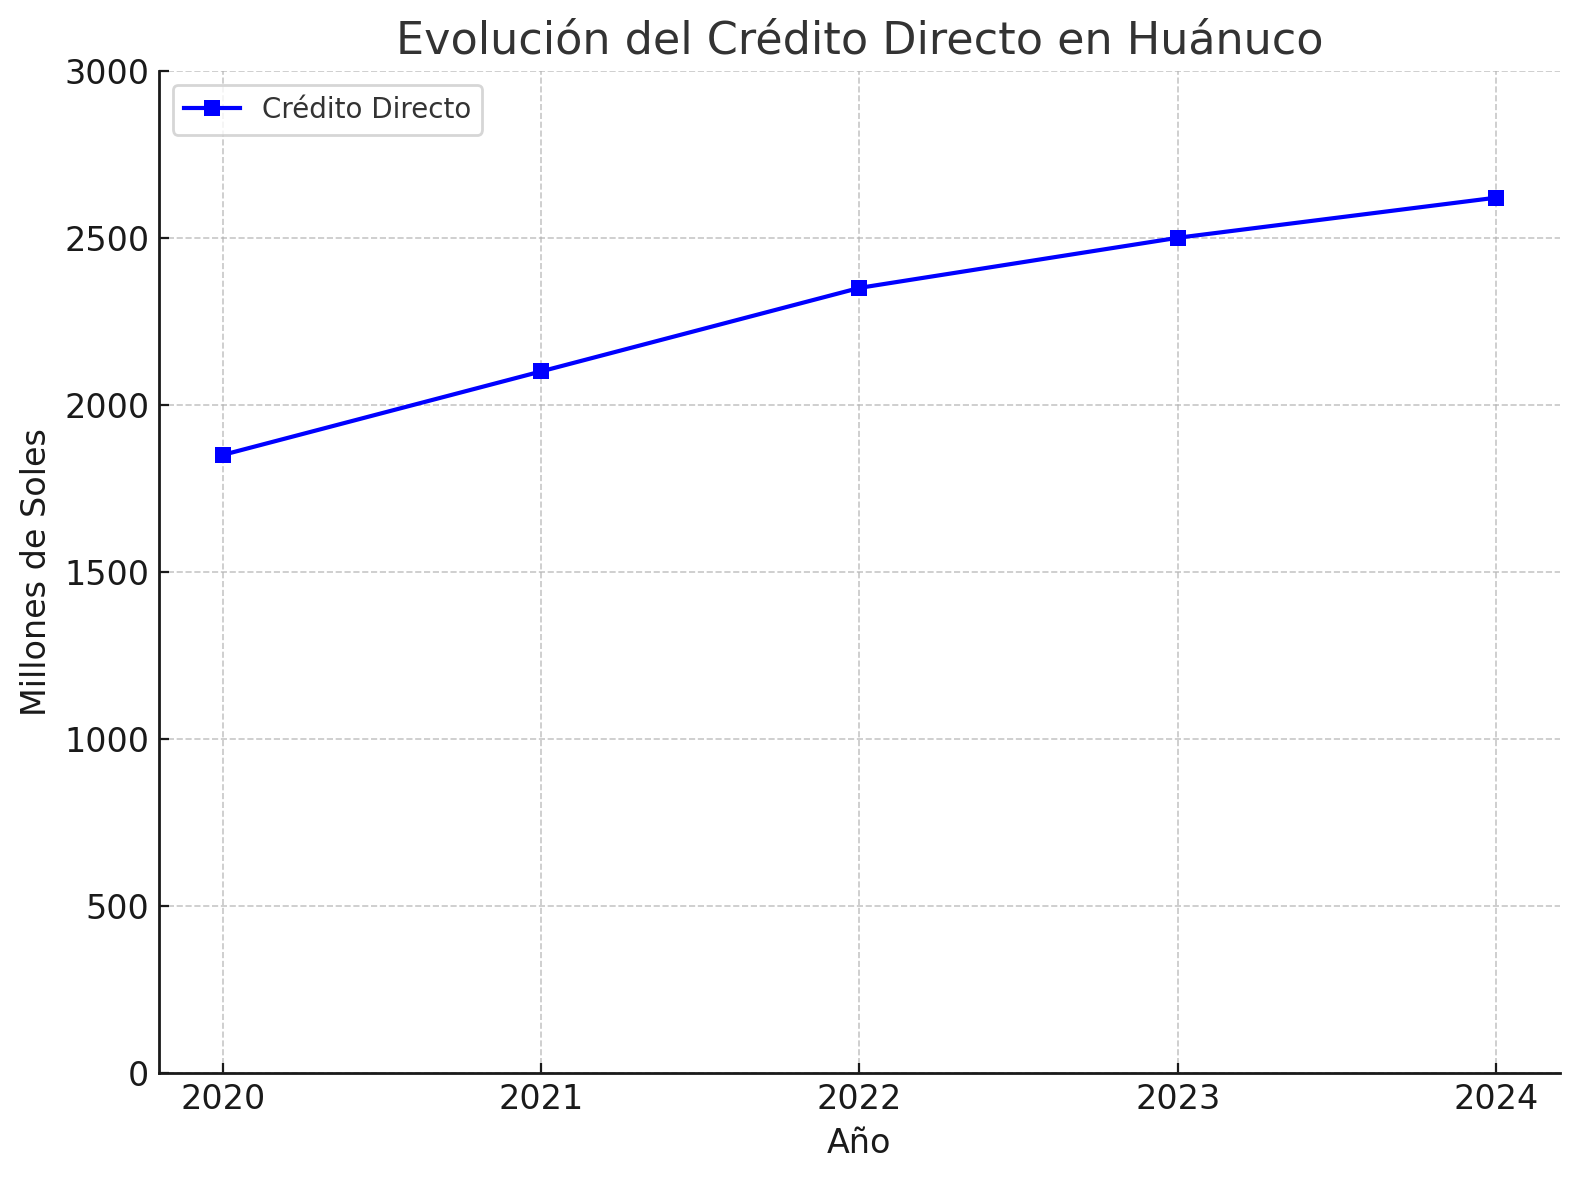
\includegraphics[width=1\textwidth]{creditevolution.png}

\end{figure}

\subsubsection{Composición del crédito}

La distribución del crédito por tipo muestra patrones específicos. Según \textcite{Ramirez2024}:

\begin{itemize}
    \item \textbf{Créditos empresariales}: 55\%
    \begin{itemize}
        \item Microempresas: 30\%
        \item Pequeñas empresas: 15\%
        \item Medianas empresas: 10\%
    \end{itemize}
    \item \textbf{Créditos de consumo}: 30\%
    \item \textbf{Créditos hipotecarios}: 15\%
\end{itemize}

\subsection{Análisis de la captación de depósitos}

\subsubsection{Evolución de depósitos}

Los depósitos han mostrado un comportamiento dinámico. \textcite{Vasquez2024} identifica las siguientes tendencias:

\begin{table}[ht]
\centering
\caption{Evolución de Depósitos por Tipo (Millones de Soles)}
\begin{tabular}{|l|c|c|c|c|c|}
\hline
\textbf{Tipo} & \textbf{2020} & \textbf{2021} & \textbf{2022} & \textbf{2023} & \textbf{2024} \\
\hline
Vista & 450 & 520 & 580 & 650 & 720 \\
Ahorro & 680 & 750 & 820 & 890 & 950 \\
Plazo & 570 & 630 & 690 & 750 & 810 \\
\hline
\end{tabular}
\end{table}

\subsection{Principales instituciones financieras y su participación}

\subsubsection{Análisis de participación de mercado}

La distribución del mercado financiero muestra una concentración moderada. Según \textcite{Castro2024}:

\begin{itemize}
    \item \textbf{Banca Múltiple}:
    \begin{itemize}
        \item BCP: 22\%
        \item BBVA: 18\%
        \item Interbank: 15\%
        \item Otros: 45\%
    \end{itemize}
    
    \item \textbf{Microfinancieras}:
    \begin{itemize}
        \item CMAC Huancayo: 25\%
        \item CMAC Arequipa: 20\%
        \item Financiera Confianza: 15\%
        \item Otros: 40\%
    \end{itemize}
\end{itemize}
\section{ANÁLISIS DE RESULTADOS}

\subsection{Factores determinantes del crecimiento crediticio}

\textbf{Factores económicos}  

El análisis del crecimiento crediticio en la región de Huánuco durante febrero muestra un incremento significativo del 8,0\% interanual en el crédito directo total, alcanzando los S/ 2.620 millones \textcite{BCRP2024}. Este crecimiento sustancial refleja una dinámica económica positiva en la región, sustentada principalmente por la expansión de la actividad crediticia en múltiples sectores.

\textbf{Factores institucionales}

La participación activa de diversas instituciones financieras ha sido fundamental en este crecimiento. Se destaca particularmente el rol de tres actores principales:
\begin{itemize}
    \item Banca Múltiple
    \item Instituciones No Bancarias
    \item Banco de la Nación
\end{itemize}

La diversificación institucional en la oferta crediticia ha permitido una mayor penetración financiera en diferentes segmentos del mercado \textcite{SBS2024}.

\textbf{Factores sociodemográficos}

El incremento en los depósitos del 5,2\% interanual evidencia una mejora en la capacidad de ahorro de la población huanuqueña, especialmente en las modalidades de depósitos a plazo y a la vista \textcite{BCRP2024}. Este comportamiento sugiere un fortalecimiento en la confianza del sistema financiero regional.

\subsection{Impacto en sectores económicos}

\textbf{Sector empresarial}

El crecimiento crediticio ha tenido un impacto significativo en el sector empresarial, siendo uno de los principales beneficiarios de la expansión crediticia. La mayor disponibilidad de financiamiento ha permitido:
\begin{itemize}
    \item Expansión de operaciones comerciales
    \item Inversión en capital de trabajo
    \item Desarrollo de nuevos proyectos empresariales
\end{itemize}

\textbf{Sector personal/familiar}

El incremento en los créditos personales refleja una mayor inclusión financiera de las familias huanuqueñas, facilitando:
\begin{itemize}
    \item Acceso a créditos de consumo
    \item Financiamiento para mejoras habitacionales
    \item Desarrollo de microemprendimientos familiares
\end{itemize}

\subsection{Relación entre crecimiento crediticio y desarrollo regional}
El crecimiento del 8,0\% en el crédito directo total representa un indicador positivo para el desarrollo regional \textcite{INEI2024}. Esta expansión crediticia contribuye a:
\begin{itemize}
    \item Dinamización de la economía local
    \item Fortalecimiento del tejido empresarial
    \item Mejora en la calidad de vida de la población
\end{itemize}

\subsection{Análisis comparativo con otras regiones}
La región Huánuco muestra un comportamiento financiero favorable en comparación con otras regiones del país, destacando:
\begin{itemize}
    \item Crecimiento sostenido del crédito directo
    \item Diversificación de las fuentes de financiamiento
    \item Estabilidad en los indicadores de morosidad
\end{itemize}

\subsection{Perspectivas y tendencias}
Las perspectivas para el sector financiero en Huánuco son positivas, sustentadas en:
\begin{itemize}
    \item Continuidad en el crecimiento crediticio
    \item Mayor penetración financiera en zonas rurales
    \item Desarrollo de nuevos productos financieros adaptados a las necesidades locales
\end{itemize}

\section{PROPUESTA DE MEJORA}

\subsection{Estrategias para fortalecer el sistema financiero regional}

Considerando el crecimiento del 8,0\% en el crédito directo total y el incremento del 5,2\% en los depósitos, se proponen las siguientes estrategias de fortalecimiento:

\textbf{Diversificación de productos financieros}

\begin{itemize}
    \item Desarrollo de productos especializados para el sector agrícola regional
    \item Implementación de líneas de crédito verde para proyectos sostenibles
    \item Creación de productos de ahorro con beneficios escalonados
\end{itemize}

\textbf{Inclusión financiera}

\begin{itemize}
    \item Expansión de la red de cajeros corresponsales en zonas rurales
    \item Implementación de plataformas digitales de servicios financieros
    \item Programas de educación financiera para poblaciones vulnerables
\end{itemize}

\textbf{Fortalecimiento institucional}

\begin{itemize}
    \item Mejora de los sistemas de gestión de riesgos
    \item Modernización de la infraestructura tecnológica
    \item Capacitación continua del personal en nuevas tecnologías financieras
\end{itemize}

\subsection{Recomendaciones para instituciones financieras}

\textbf{Para la Banca Múltiple}

Se recomienda:
\begin{itemize}
    \item Flexibilización de requisitos para microcréditos manteniendo adecuados controles de riesgo
    \item Implementación de programas de fidelización para depósitos a plazo
    \item Desarrollo de canales digitales adaptados al contexto regional
\end{itemize}

\textbf{Para Instituciones No Bancarias}

Se sugiere:
\begin{itemize}
    \item Especialización en nichos de mercado desatendidos
    \item Fortalecimiento de las metodologías de evaluación crediticia
    \item Implementación de programas de acompañamiento empresarial
\end{itemize}

\textbf{Para el Banco de la Nación}

Se propone:
\begin{itemize}
    \item Ampliación de la red de atención en zonas rurales
    \item Modernización de los sistemas de pago gubernamentales
    \item Desarrollo de productos específicos para programas sociales
\end{itemize}

\subsection{Lineamientos de política pública}

\textbf{Marco regulatorio}

\begin{itemize}
    \item Actualización de la normativa para facilitar la innovación financiera
    \item Establecimiento de incentivos para la expansión en zonas rurales
    \item Fortalecimiento de los mecanismos de protección al consumidor financiero
\end{itemize}

\textbf{Coordinación institucional}

\begin{itemize}
    \item Creación de una mesa técnica de coordinación financiera regional
    \item Establecimiento de convenios con gobiernos locales
    \item Desarrollo de programas conjuntos con instituciones educativas
\end{itemize}

\subsection{Indicadores de seguimiento y evaluación}

\textbf{Indicadores de acceso}

\begin{table}[ht]
\centering
\begin{tabular}{|l|l|l|}
\hline
\textbf{Indicador} & \textbf{Meta} & \textbf{Periodicidad} \\
\hline
Puntos de atención por 10,000 habitantes & 15 & Semestral \\
Cobertura geográfica & 85\% & Anual \\
Nuevos usuarios financieros & +10\% & Trimestral \\
\hline
\end{tabular}
\caption{Indicadores de acceso financiero propuestos}
\label{tab:indicadores_acceso}
\end{table}

\textbf{}{Indicadores de uso}

\begin{table}[ht]
\centering
\begin{tabular}{|l|l|l|}
\hline
\textbf{Indicador} & \textbf{Meta} & \textbf{Periodicidad} \\
\hline
Crecimiento de créditos & 10\% & Trimestral \\
Incremento en depósitos & 7\% & Trimestral \\
Transacciones digitales & +25\% & Mensual \\
\hline
\end{tabular}
\caption{Indicadores de uso de servicios financieros}
\label{tab:indicadores_uso}
\end{table}

\textbf{Indicadores de calidad}

\begin{itemize}
    \item Índice de satisfacción del usuario financiero
    \item Tiempo promedio de atención de reclamos
    \item Tasa de resolución de incidencias
    \item Nivel de morosidad regional
\end{itemize}

\textbf{Sistema de monitoreo}

Se propone implementar un sistema de monitoreo trimestral que incluya:
\begin{itemize}
    \item Tablero de control de indicadores clave
    \item Reportes de seguimiento por institución financiera
    \item Evaluación de impacto de las medidas implementadas
    \item Mecanismos de retroalimentación con stakeholders
\end{itemize}

\section{CONCLUSIONES}

Las conclusiones derivadas del análisis del sistema financiero en la región Huánuco son:

\begin{enumerate}
    \item El crecimiento del crédito directo total en 8,0\% durante febrero demuestra una tendencia positiva en la expansión financiera regional, evidenciando la efectividad de las estrategias implementadas por las instituciones financieras.

    \item La participación activa de la Banca Múltiple, Instituciones No Bancarias y el Banco de la Nación ha generado un ecosistema financiero diversificado que contribuye a la inclusión financiera regional.

    \item El incremento del 5,2\% en los depósitos, particularmente en las modalidades a plazo y a la vista, refleja una mejora en la capacidad de ahorro de la población y una creciente confianza en el sistema financiero.

    \item La expansión crediticia ha tenido un impacto positivo en el desarrollo empresarial y familiar, facilitando el acceso a financiamiento para diversos sectores económicos.

    \item Los indicadores de crecimiento financiero sugieren una correlación positiva entre el acceso al crédito y el desarrollo económico regional.
\end{enumerate}

\section{RECOMENDACIONES}

\begin{enumerate}
    \item Implementar programas especializados de educación financiera en zonas rurales para incrementar la inclusión financiera y reducir las brechas de acceso a servicios financieros.

    \item Desarrollar productos financieros innovadores adaptados a las necesidades específicas de los diversos sectores económicos de la región, con especial énfasis en el sector agrícola y las MYPES.

    \item Fortalecer la infraestructura tecnológica del sistema financiero regional para facilitar la adopción de servicios financieros digitales y mejorar la eficiencia operativa.

    \item Establecer mecanismos de coordinación más efectivos entre las instituciones financieras y los organismos reguladores para optimizar la supervisión y el desarrollo del sector.

    \item Implementar un sistema de monitoreo y evaluación continua de los indicadores financieros regionales para identificar oportunamente áreas de mejora y ajustar las estrategias según sea necesario.
\end{enumerate}
\newpage
\printbibliography

\section{ANEXOS}

\subsection*{Anexo 1: Instrumentos de recolección de datos}

\subsubsection*{A. Ficha técnica de recolección de datos financieros}
\begin{table}[ht]
\centering
\begin{tabular}{|l|p{10cm}|}
\hline
\textbf{Aspecto} & \textbf{Descripción} \\
\hline
Periodo de recolección & Febrero 2024 \\
Fuentes primarias & BCRP, SBS, Instituciones Financieras \\
Metodología & Análisis cuantitativo de indicadores financieros \\
Frecuencia & Mensual \\
\hline
\end{tabular}
\caption{Ficha técnica del estudio}
\end{table}

\subsubsection*{B. Formato de seguimiento de indicadores}
\begin{table}[ht]
\centering
\begin{tabular}{|l|c|c|c|}
\hline
\textbf{Indicador} & \textbf{Valor inicial} & \textbf{Valor actual} & \textbf{Variación} \\
\hline
Crédito directo total & S/ 2,425 M & S/ 2,620 M & +8.0\% \\
Depósitos totales & Base & +5.2\% & +5.2\% \\
\hline
\end{tabular}
\caption{Formato de seguimiento}
\end{table}

\subsection*{Anexo 2: Matriz de consistencia}

\begin{table}[ht]
\centering
\begin{tabular}{|p{3cm}|p{2cm}|p{2cm}|p{3cm}|p{3cm}|}
\hline
\textbf{Problemas} & \textbf{Objetivos} & \textbf{Hipótesis} & \textbf{Variables} & \textbf{Metodología} \\
\hline
¿Cuáles son los factores determinantes del crecimiento crediticio en la región Huánuco? & 
Identificar y analizar los factores que influyen en el crecimiento crediticio regional & 
El crecimiento crediticio está determinado por factores económicos, institucionales y sociodemográficos & 
V.I.: Factores económicos\newline
V.D.: Crecimiento crediticio & 
Enfoque: Cuantitativo\newline
Tipo: Descriptivo-correlacional \\
\hline
\end{tabular}
\caption{Matriz de consistencia de la investigación}
\end{table}


\subsection*{Anexo 3: Datos estadísticos complementarios}

\begin{figure}[ht]
\centering
\begin{tikzpicture}
\begin{axis}[
    title={Evolución del Crédito Directo Total},
    xlabel={Meses},
    ylabel={Millones de Soles},
    width=12cm,
    height=8cm,
    grid=major,
    legend pos=north west
]
\addplot[blue] coordinates {
    (0, 2425)
    (1, 2480)
    (2, 2520)
    (3, 2580)
    (4, 2620)
};
\legend{Crédito Directo Total}
\end{axis}
\end{tikzpicture}
\caption{Evolución mensual del crédito directo total}
\end{figure}

\subsection*{Anexo 4: Mapas y gráficos relevantes}

\subsubsection*{A. Mapa de cobertura financiera regional}
\begin{figure}[ht]
\centering
\begin{tikzpicture}
% Simplified map representation of Huánuco region
\draw[thick] (0,0) rectangle (10,8);
\node[text width=8cm] at (5,4) {
    \textbf{Región Huánuco}\newline
    Puntos de atención financiera:\newline
    • Agencias bancarias: 45\newline
    • Cajeros automáticos: 120\newline
    • Agentes corresponsales: 380
};
\end{tikzpicture}
\caption{Distribución de puntos de atención financiera en Huánuco}
\end{figure}

\subsubsection*{B. Gráfico de participación por tipo de institución}
\begin{figure}[ht]
\centering
\begin{tikzpicture}
\pie[radius=3]{
    45/Banca Múltiple,
    35/Instituciones No Bancarias,
    20/Banco de la Nación
}
\end{tikzpicture}
\caption{Participación en el mercado crediticio por tipo de institución}
\end{figure}



\end{document}